% Template for ICIP-2019 paper; to be used with:
%          spconf.sty  - ICASSP/ICIP LaTeX style file, and
%          IEEEbib.bst - IEEE bibliography style file.
% --------------------------------------------------------------------------
\documentclass{article}
\usepackage{spconf,amsmath,graphicx}

\newtheorem{definition}{Definition}
\usepackage[utf8]{inputenc}
\usepackage{graphicx}
\usepackage{float}
\usepackage{pgfplots}
\pgfplotsset{
  compat=1.13,
}


% Example definitions.
% --------------------
\def\x{{\mathbf x}}
\def\L{{\cal L}}

% Title.
% ------
\title{GOOGLE'S SEARCH ALGORITHM AND PRIVACY ISSUES}
%
% Single address.
% ---------------
\name{Christian Bojko, David Pape}
\address{Universität Salzburg}
%
% For example:
% ------------
%\address{School\\
%	Department\\
%	Address}
%
% Two addresses (uncomment and modify for two-address case).
% ----------------------------------------------------------
%\twoauthors
%  {A. Author-one, B. Author-two\sthanks{Thanks to XYZ agency for funding.}}
%	{School A-B\\
%	Department A-B\\
%	Address A-B}
%  {C. Author-three, D. Author-four\sthanks{The fourth author performed the work
%	while at ...}}
%	{School C-D\\
%	Department C-D\\
%	Address C-D}
%
\begin{document}
%\ninept
%
\maketitle
%
\begin{abstract}
Googles Suchalgorithmen werden laufend erneuert und verbessert. Dabei startet eine Suche weit vor dem eigentlich eingeben eines Suchwortes und zwar bereits mit dem Sammeln der Daten von Websiten.
Google's Privacy Probleme betreffen fast alle ihrer Produkte. Unter anderem gibt es Datenschutz und Privatsphäre Problematiken bei Google Browser Chrome, der Google Suchmaschine, dem Smartphone OS Android, Cookies und Google Mail. Da die meisten Dienste von Google in ihrem Bereich den Höchsten oder einen der Höchsten Marktanteile besitzten, ist das Sammeln von Daten der User umso problematischer. Wir nehmen diese Probleme etwas genauer unter die Lupe und zeigen welche Daten gesammelt und auch verkauft werden um daraus Profit zu machen.
\end{abstract}
%
\begin{keywords}
google, search, privacy
\end{keywords}
%


\section{Introduction}

Google beschreibt die Herausforderungen eines modernen Web-Suchalgorithmus wie folgt:\cite{googs}:

\begin{quote}
In a fraction of a second, Google’s Search algorithms sort through hundreds of billions of webpages in our Search index to find the most relevant, useful results for what you’re looking for.
\end{quote}

Es ist somit offensichtlich, dass hier interessante technische (und soziale) Herausforderungen bestehen. Wir betrachten zunächst die einzelnen Schritte, die Google unternimmt, um schlussendlich Suchergebnisse zu präsentieren, und geben schlussendlich Bedenken in Hinsicht auf die Privatsphäre der Nutzer.

\section{Funktionsweise des Algorithmus}

\subsection{Crawling}

Das Crawling ist der erste Schritt in der Pipeline von Googles Suchalgorithmus. Der Crawling-Prozess beginnt mit einer Liste von Webadressen aus früheren Crawls und Sitemaps, die der sogenannte Google-Bot nutzt, um Websites zu besuchen.

\begin{definition}[Sitemap]
Eine Datei, in der Informationen über die Seiten, Videos und anderen Dateien und deren zusammenhang stehen. Sie helfen der Google-Suche wichtige Informationen von der Website leichter zu finden.
\end{definition}

Sitemaps werden von den Besitzern der Webseite extra erstellt, um Google beim Crawlen der Webseite zu helfen. Die Motivation dabei ist, dass ein besseres Ranking erlangt wird, je nachdem wie gut Google-Bot den Inhalt der Seite einschätzen kann.

Google-Bot folgt beim Crawlen auch Links zu neuen Websites und springt sozusagen immer weiter.

Weitere Programme werten dann den Inhalt aus und verarbeiten die Daten.

\subsection{Indexing}

Die im Crawling-Prozess gesammelte Information wird in einem gigantischen Index gesammelt. Der Index ist über 100 Petabyte groß\cite{si} und ist entsprechend auf sehr viele Rechner verteilt. Die enthaltenen Informationen sollen widerspiegeln, was das Thema einer Seite ist.

\subsection{Ranking}

Das Ziel ist, die \textit{Relevanz} der Suchergebnisse für den Nutzer zu maximieren. Dabei entstehen einige Herausforderungen.

Zunächst fällt auf, dass sich Nutzer oft bei der Eingabe einer Suchanfrage vertippen. Dieses Problem ist sicher nicht besser geworden, seitdem über 60\% der Suchanfragen von Smartphones kommen\cite{mq}. Tippfehler zu beheben, ist nicht einfach - oft gibt es mehrere Wörter, die eine naheliegende und passende Korrektur wären. Man kann sich manchmal auch nicht sicher sein, ob überhaupt ein Tippfehler vorliegt oder dies die beabsichtigte Anfrage des Nutzers ist, insbesondere bei Akronymen.

Google löst dieses Problem durch die Einblendung des bekannten ``Did you mean:''.

Ein weiteres Problem ist, dass Nutzer zunehmend mit Natural Language Queries suchen. Dies bedeutet, dass nicht nach konkreten Datenpunkten wie ``wm sieger 2014'' gesucht wird, sondern nach einem vollständigen Satz wie ``wer hat die wm 2014 gewonnen''. Die Interpretation solcher Suchanfragen bildet eine weitere Herausforderung.

Insbesondere liegt in menschlichen Sprachen oft Mehr- deutigkeit vor. Dabei gibt Google folgende Beispiele\cite{sa}:

\begin{itemize}
    \item ``how to \textbf{change} a light bulb''
    \item ``does post office \textbf{change} foreign currency''
    \item ``how to \textbf{change} laptop brightness''
\end{itemize}

Dies kompliziert die Interpretation von Natural Language Queries weiter.

Schlussendlich muss unterschieden werden, ob aktuelle Information gesucht wird oder nicht. Zum Beispiel wollen Nutzer wahrscheinlich den aktuellen Kurs sehen, wenn sie nach ``apple aktie'' suchen, und nicht irgendeinen vergangenen. Google löst dieses Problem unter Anderem dadurch, dass aktuelle Information geliefert wird, wenn ein Begriff "trending" ist, d.h. mehr Leute als üblich suchen diesen Begriff momentan.

Wichtig ist auch der Kontext: wenn jemand nach ``burgerista öffnungszeiten'' sucht, dann sollte der Standort des Nutzers beachtet werden, um ihm möglichst die Öffnungszeiten seines lokalen Burgerista zu liefern.

\subsection{Geschichte von Googles Suchalgorithmen}
        
Google hat den Suchalgorithmus kontinuierlich über die Jahre verbessert, um die erwähnten Herausforderungeb zu lösen. Wir geben nun einen Überblick über die Evolution von dem Algorithmus.
        
\subsubsection{PageRank}

PageRank war der ursprüngliche Suchalgorithmus von Google in den 90ern. Die Neuheit von PageRank war, dass Seiten nach der Anzahl \textit{Backlinks} gereiht wurden\cite{pr}.

\begin{definition}[Backlink]
Eine Seite $S$ hat $n$ Backlinks, wenn es $n$ Links zu $S$ gibt.
\end{definition}

In PageRank wurde jedem Backlink auch ein Gewicht zugewiesen - wenn die Seite, von der der Backlink stammt, selbst wichtig ist, dann zählt ein solcher Backlink mehr als ein Backlink von einer unwichtigen Seite.

\subsubsection{Missbrauchspotenzial}

Da Google akademische Ursprünge hat, war der PageRank Algorithmus öffentlich\cite{pr}, und somit war es trivial, mit sog. Linkfarmen für den Algorithmus zu optimieren. Dies musste mit künftigen, nicht-öffentlichen Updates bekämpft werden.

\subsection{Updates zum Suchalgorithmus}

Mit der Zeit wurden viele Updates zum Algorithmus eingeführt, die die genannten Probleme beheben sollten.

\subsubsection{Panda (2011)}

Panda sollte die \textit{Qualität} von Webseiten automatisch be- werten\cite{ah}. Dabei wurden folgende Faktoren herangezogen:

\begin{itemize}
    \item Ist die SEO sauber? (Metadaten, Sitemap)
    \item Formulierung der Texte
    \item Qualität der Grafiken
    \item Sind die Unterseiten einander ähnlich?
    \item Wie lange bleiben die Besucher im Allgemeinen?
\end{itemize}

\subsubsection{Penguin (2012)}

Penguin war ein Update, um sog. ``Black Hat SEO'' abzu- werten\cite{ah}. Black Hat SEOO ist die Ausnutzung von Eigenschaften des Suchalgorithmus, wie z.B. in genannten Linkfarmen. Penguin hat dazu betrachtet, ob Seiten:

\begin{itemize}
    \item Texte künstlich mit übermäßig vielen Keywords anreichern
    \item für die Nutzer unsichtbare Texte in die Seite einzubauen, um mehr Keywords unterzubringen (z.B. mit white-on-white text)
\end{itemize}

\subsubsection{Hummingbird (2013)}

Hummingbird erlaubte Suchen nicht nur per Keyword, sondern per Semantik\cite{ah}. Es sollte also zur Erfüllung von Natural Language Queries nutzen: wie bereits genannt, könnte man nun statt ``wm sieger 2014'' nach ``wer hat die wm 2014 gewonnen'' suchen und auf sinnvolle Ergebnisse hoffen.

\subsubsection{RankBrain (2015)}

RankBrain war ein entscheidendes Update für den Algorithmus, in dem ML/AI-Technologien erstmals als Kerntechnologien für das Ranking eingesetzt wurden\cite{ah}\cite{ahr}. Das Ziel dabei war primär die Bearbeitung von Suchanfragen, die Google zuvor noch nie bekommen hat. Solche Suchanfragen bilden 15\% der Anzahl aller täglichen Suchanfragen, die Google bekommt\cite{nqs}, und sind somit ein wichtiges Ziel.

AI wurde dabei eingesetzt, um die Semantik neuer Anfragen zu analysieren. So sollten dann ähnliche, bereits beantwortete Anfragen zur Hilfe gezogen werden können, um neue Anfragen besser zu bearbeiten\cite{ahr}.

\subsection{Suchalgorithmus heute}

Heutzutage ist der Suchalgorithmus also viel klüger geworden und versteht auch den Inhalt der Seiten. Damit ist Black Hat SEO weniger effektiv. Weiters ist die genaue Funktionsweise nicht mehr öffentlich. Bekannt ist aber, dass u.a. folgende Variablen berücksichtigt werden:

\begin{itemize}
    \item Standort
    \begin{itemize}
        \item Eine Suche nach ``bicycle repair shop'' in Paris sollte ganz andere Ergebnisse liefern als eine in Tokio. 
        \item Allerdings sollte dies für eine Suche nach ``last nobel prize winner'' nicht der Fall sein.
    \end{itemize}
    \item Datum und Zeit
    \begin{itemize}
        \item Eine Suche nach ``wm sieger'' sollte den Sieger der \textit{letzten} WM finden.
    \end{itemize}
    \item Sprache
    \item Vorherige Suchanfragen
    \begin{itemize}
        \item Hieraus kann wertvoller Kontext gewonnen werden
        \item Wiederholte Anfragen bedeuten, dass vorherige Suchen nicht das richtige Ergebnis geliefert haben
    \end{itemize}
    \item Gerät des Nutzers
    \begin{itemize}
        \item Hauptsächlich geht es um Desktop, Tablet oder Mobile
        \item Beispielsweise werden ``mobile-friendy'' Seiten bevorzugt, wenn der Nutzer auf einem Mobilgerät ist.
    \end{itemize}
\end{itemize}

\section{Privacy-Probleme}

\subsection{Cookies}
Ein Cookie ist einfach eine Textinformation die vom Browser auf dem Rechner abgespeichert wird. Es wird entweder per Script erstellt oder vom Webserver an der Browser gesendet und so gespeichert. Jedesmal wenn eine Website geöffnet wird, werden die Cookies geupdatet und neue Information darin gespeichert. Ein Cookie hat dabei eine Eindeutige ID die den Nutzer immer identfiziert. Daneben können noch viele weitere Daten wie zum Beispiel Name, Adresse, Email oder Telefonnummer gespeichert werden. Die wichtigste Regel dabei ist, dass jede Website nur ihr eigenes Cookie vom User auslesen kann. Wie diese Regel aber umgangen werden kann, kommt später. Google platziert eins oder mehrere Cookies auf den Rechner des Users und kann dadurch Sucherverläufe, Browserverläufe abspeichern.  Wenn das ganze noch mit einem Google Konto verbunden ist, werden diese Cookies darauf noch abgespeichert und wenn man sich auf einem neuen Rechner anmeldet, hat er diese Cookies natürlich wieder zur Verfügung. 2016 wurden die Datenschutzrichtlinien soweit geändert, dass es jetzt nicht mehr ersichtlich ist, ob und wann diese Cookies gelöscht werden. Natürlich können solche Informationen bei Strafrechtlicher Verfolgung an die Polizei weitergeleitet werden.

\subsection{Tracking}
Ein sehr starkes Tool zur Überwachung eines users ist das so genannte Tracking. Wobei es schwer ist zu beweisen ob das stattfindet, ist es dennoch Erwähnenswert. Dadurch dass Google viele Tools und Dienste im World Wide Web laufen hat, ist es schon fast unvermeidlich auf irgend eine Website ohne der Hilfe von Google zu kommen. Dienste wie Analytics, Play Services, reCAPTCHA, Google Fonts. Durch diese Tools ist es Google möglich dass man die Route die eine Abfrage eines Users nimmt zu ermitteln. Dabei ist es schwer überhaupt einen Überblick zu bekommen wohin die Daten jeweils gehen.

\subsection{Captcha}
Ein kleines Beispiel wie die Regel, dass Cookies nur von der eigenen Website, gelesen und geändert werden kann dadurch Umgangen werden, dass das reCaptcha, was auf einer anderen Website genutzt wird, ein Dienst ist, der als Domain www.google.com verwendet. Somit das das Captcha alle Informationen von der Website auf der es ist und kann das eigentliche Google Cookie eines User anpassen je nachdem wo das Captcha gerade genutzt wurde.

\subsection{Google Mail}
Ein Weiterer Google Dienst der sehr viel genutzt wird, ist Google Mail. Der Emaildienst, den jeder kennt und der rund 1,5 Milliarden Accounts hat, ist zwar gratis für jeden User aber dieser Dienst wird hauptsächlich für Marketing Zwecke genutzt. Laut Google werden Mails nie von anderen Menschen gelesen, was aber nicht bedeutet dass nicht Computer und Algorithmen die Mails lesen und analysieren um ein genaueres Bild eines Users und dadurch besser angepasste Werbung zu schalten. Zum Beispiel können Emails von Amazon oder anderen Lieferdiensten ausschlag geben, was, wie oft ein User etwas bestellt und wieviel Geld er dafür ausgibt. Andererseits können auch Private Mails Auskunft geben wie es dem User geht etc.


    

Dazu gibt es ein gutes Zitat von Eric Schmidt, Google CEO 2010

\begin{quote}
     We know where you are, we know where you’ve been, We can more or less know what you’re thinking about.
\end{quote} 
Dieses Zitat gibt einen sehr guten Eindruck über die Idee hinter Google.\newline

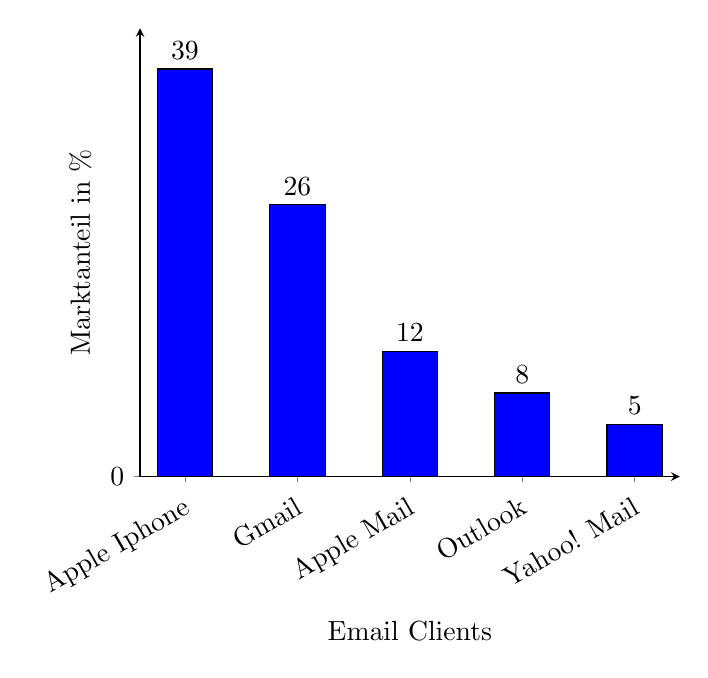
\begin{tikzpicture}
  \begin{axis}[
    ybar,
    bar width=20pt,
    %
    nodes near coords,
    nodes near coords align=above,
    point meta=rawy,
    %
    axis x line=bottom,
    axis y line=left,
    ymajorgrids=true,
    %
    ylabel=Marktanteil in \%,
    ymin=0,
    ytick={0,50,100},
    enlargelimits=auto,
    %
    xlabel= Email Clients,
    symbolic x coords ={Apple Iphone,Gmail,Apple Mail,Outlook,Yahoo! Mail},
    x tick label style={rotate=30,anchor=north east},
    ]

    \addplot[fill=blue] coordinates {
      (Apple Iphone,39)
      (Gmail,26)
      (Apple Mail,12)
      (Outlook,8)
      (Yahoo! Mail,5)
    };
  \end{axis} 
\end{tikzpicture}

\subsubsection{Third-Party Apps}
Ein weiterer Punkt bei Gmail ist das seit 2014 Third-Party Entwickler Zugang zur Gmail API bekommen haben und dadurch Software für die Platform erstellen können. Diese Software sind meist Aufgabenmanager oder Apps zum Signieren von Dokumenten. Das Problem dahinter besteht darin, dass diese Apps beim installieren automatisch zugriff auf Emails bekommen.

Im Wall Street Journal 2018 gab es einen Beitrag über einen Vorfall wo Angestellter eines solchen Drittanbieters rund 8000 Emails Gelesen wurden um ihre Algorithmen zu verbessern.

\subsection{Google Chrome}
Google Chrome ist der meist verbreiteste Browser. Dabei geht es hauptsächlich um die Suchleiste und wie diese Funktioniert. Bei Chrome ist die Suchleiste eine Omnibar da sie die Adresse und das Suchen verbindet. Dabei werden aber, um natürlich die besten Sucheregebnise liefern zu können in Echtzeit die Wörter/Buchstaben die man tippt an den Server übertragen. Der Gründer von Fluid New Media, Ahad Bokhari, fand durch das Testen des Browsers im Debug-Proxy Mode heraus, dass bei fast jedem Tastenschlag mit dem Server kommuniziert wird. Diese Informationen und anhand der bereits bestehenden cookies können dabei eine sehr genaue Suche garantieren.


\begin{figure}[htb]
    \begin{minipage}[b]{1.0\linewidth}
      \centering
      \centerline{\includegraphics[width=8.5cm]{browsermarketshare.png}}
      \centerline{https://gs.statcounter.com/browser-market-share}\medskip
    \end{minipage}

    \begin{minipage}[b]{1.0\linewidth}
      \centering
      \centerline{\includegraphics[width=8.5cm]{googlesearchmarketshare.png}}
    \end{minipage}
    \caption{Marktanteil von Browsern und Suchmaschinen\cite{bms}\cite{sems}}
\end{figure}


\subsection{Android}
Das Betriebssystem Android ist mit 72\% Marktanteil und mit rund 2,5 Milliarden aktiven Geräten das weitaus meist verbreitete Betriebssystem für Smartphones. Dabei gibt es einige Lücken die die Privatsphäre eines Users stark angreifen. 

The Associated Press hat zum Beispiel herausgefunden, dass auch ohne Standortinformationen eine Standortspeicherung stattfindet und Google immer noch zugriff auf den Standort hat. Dies geschieht meist über LTE/Wlan etc.
Ein weiteres Problem ist dass jede App theoretisch die Möglichkeit hat den screen state abzufragen. Das ist auch ohne explizite Berechtigung möglich. Dadurch kann eine App sich ein Bild machen, wann ein User wach ist und wann nicht und wie oft er am Tag sein Handy entsperrt. 

Weiters kann eine App auch Wifi und Mobildatennutzung überwachen. Daraus kann man schließen ob der User gerade Videos Streamt oder Nachrichten Sendet etc.

Eine App kann auch eine Liste mit allen anderen installierten Apps einsehen. Dadurch kann man auch wieder das Bild eines Users verbessern, da man weiß ob er viel Spiele spielt, viele Sport Apps hat etc. Das letzte ist dass Apps den Winkel, die Richtung und ob das Telefon bewegt wird auslesen können. Verknüpft man das wieder mit all den anderen Daten ist es relativ leicht einen User einzuschätzen.

% References should be produced using the bibtex program from suitable
% BiBTeX files (here: strings, refs, manuals). The IEEEbib.bst bibliography
% style file from IEEE produces unsorted bibliography list.
% -------------------------------------------------------------------------
\bibliographystyle{IEEEbib.bst}
\bibliography{strings,refs}

\end{document}
